\chapter{Data}

There are 3 types of data we can use to test the capability of the script. Iridium flares can be predicted before hand, allowing one to prepare to collect their data. NASA data provide a steady source of fireball events to access along with their data to compare to. Finally, fireball events detected by D6 will be tested, 

\section{Iridium Flares}

The next step in testing out the script is to run it in conjunction with video collected directly from D6. A simple way to do this is to run it against a video clip of an iridium flare that D6 captured. There are two benefits of testing against an iridium flare. First, iridium flares are monitored online and their max magnitudes are recorded. We can find the maximum value from our light curve and compare it to that maximum magnitude. Second, the light curves from iridium flares are very smooth. This makes it easy to notice any discrepancies in individual frames. We have collected two iridium flare events using D6. 

On *some date in fall*, D6 was able to capture an iridium flare going over Collins Hall at Willamette University in Salem, Oregon. The first frame of this event is shown as Figure~\ref{fig:iridium}. 

\begin{figure}[ht!]
	\centering
	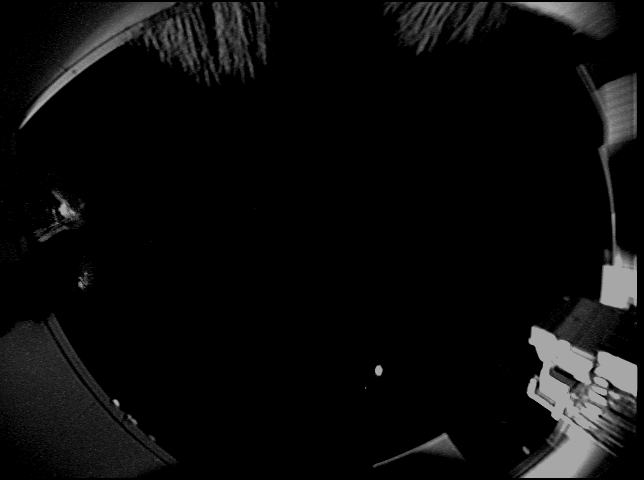
\includegraphics[width=0.6\linewidth]{iridium.png}
	\caption{The first iridium flare captured by D6 at Willamette University.}
	\label{fig:iridium}
\end{figure}

The event was analyzed by the script, producing an accurate-looking light curve. This is shown in Figure~\ref{fig:iridiumcurve}

\begin{figure}[ht!]
	\centering
	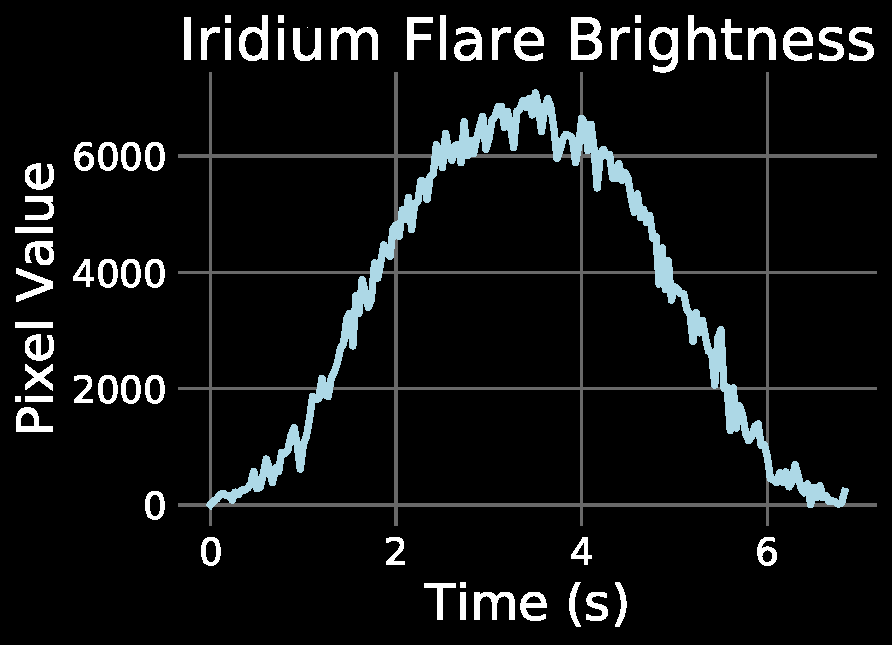
\includegraphics[width=0.6\linewidth]{/home/luke/Data/IridiumFlare/IridiumMag.pdf}
	\caption{Name}
	\label{fig:iridiummag}
\end{figure}

\begin{figure}[ht!]
	\centering
	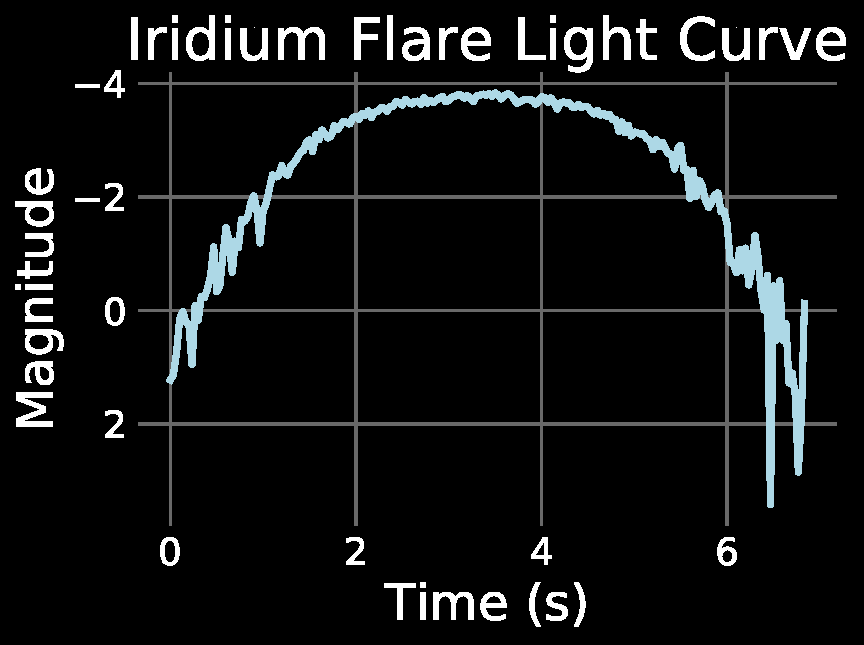
\includegraphics[width=0.6\linewidth]{/home/luke/Data/IridiumFlare/IridiumCurve.pdf}
	\caption{The light curve of the iridium flare event.}
	\label{fig:iridiumcurve}
\end{figure}

The first thing to check is if it qualitatively agrees with visual inspect of the event's video. The iridium flare's brightness seems to dramatically increase before dimming away. Both Figure~\ref{fig:iridiumcurve} and Figure~\ref{fig:iridiummag} agree with that assessment. So in a general sense, the photometry program is capable of following the event.

Some issues did emerge from this event, however. Ideally, we would like to be able to compare the maximum magnitude from the light curve our program created to the recorded maximum magnitude of the event. Unfortunately, the iridium flare was so bright that it oversaturated our camera. This can be seen in Figure~\ref{fig:ObjectPlot055}.

\begin{figure}[ht!]
	\centering
	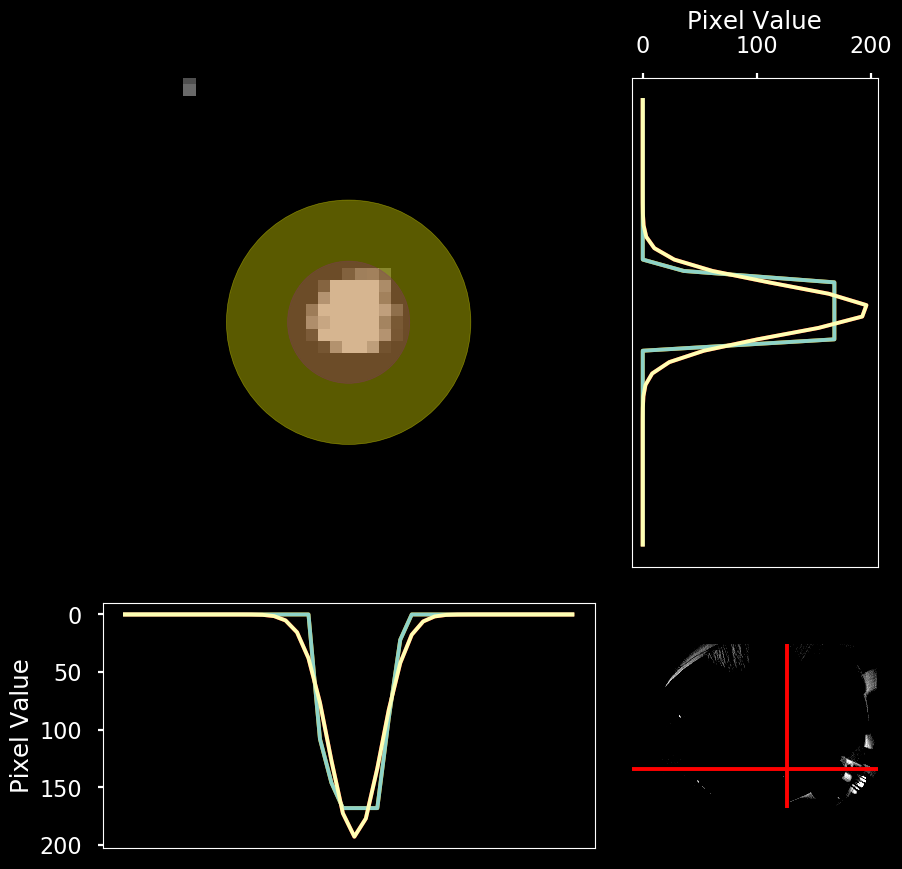
\includegraphics[width=0.6\linewidth]{ObjectPlot055.png}
	\caption{ObjectPlot055}
	\label{fig:ObjectPlot055}
\end{figure}

Figure~\ref{fig:ObjectPlot055} allows us to see that the center of event is too bright for our camera's sensors. As a result, we are unable to find the current maxium magnitude of that iridium flare event. This saturation also explains why the peaks in Figure~\ref{fig:iridiumcurve} and Figure~\ref{fig:iridiummag} last for a substantial portion of the event; the true peak brightness isn't visible on those graphs. 

Another issue that is apparent in the iridium flare data is an excess of noise insections of the data. Specifically, the noise at the end of the event appears most jarring in Figure~\ref{fig:iridiummag}. When the event nears its end, the signal to noise greatly decreases. This noise is a result of the background light that has already been mentioned. Since the event is at its end, it is becoming incredibly dim, and in its last moments its signal is basically equal with the background light around it. Since the background light value we are using is the average of the area around the event, there arises occasions where the pixels of the event are smaller than the background light at this stage. This creates a magnitude that is the resultant of a log of an incredibly small, or even negative number. Since taking the logarithm of a negative error would break the program if left untreated, those values are set to 0. So, at the end of an event before the program no longer detects any trace, it has a few data points that are incredibly smaller, whose tiny size is magnified (this seems oxymoronic???) in the logarithmic-based light curve. While not aesthetically pleasing, this small values do not affect our results, as our results will be based off integrating the intensity along the light curve.

Iridium flares are somewhat useful pseudo-meteors, but ultimately the program needs to show that it can successfully track actual meteors. When running the program on an iridium flare event, the tracking algorithm is not challenged greatly; the flare's light was at a relatively constant position on the camera's frames. Meteor events that do move far across the screen pose a new challenge for the program.

\section{Comparison to NASA Data}

The methods section provided an example of an acquired light curve from the completion of analysis from a NASA video clip. By running the script against clips from NASA, we can confirm that the script is working by comparing it to NASA's light curves provided with the videos. The collected data and results of this test are discussed below.

The first event that we acquired from NASA's database was one that occurred on March 21, 2018, by one of their cameras stationed at LOCATION. The video was downloaded alongside their infographic of data involving the event. This infographic, displayed as Figure~\ref{fig:infographic} contains the light curve of the event in the top right corner. 

\begin{figure}[ht!]
	\centering
	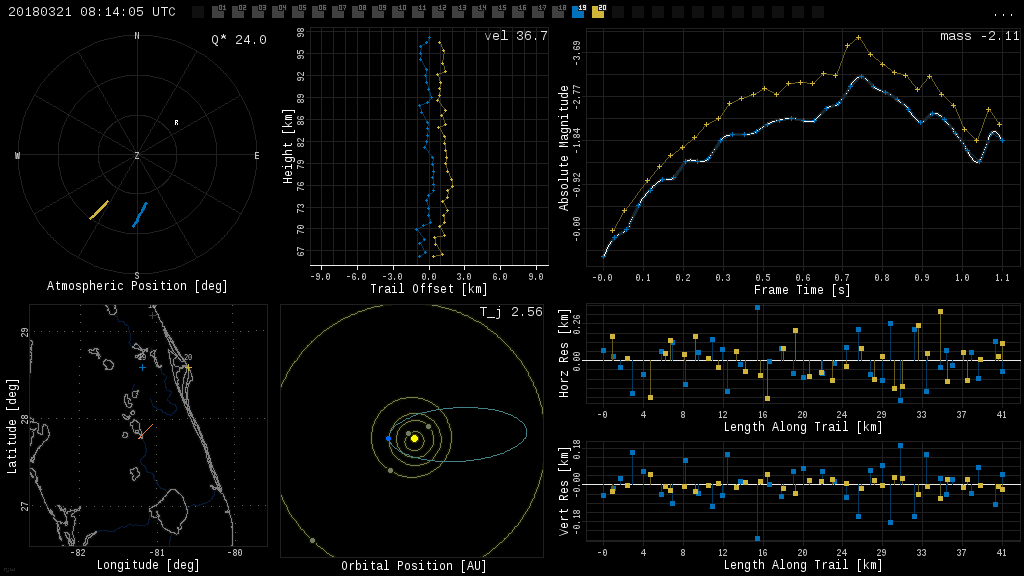
\includegraphics[width=0.8\linewidth]{infographic.png}
	\caption{The light curve NASA attained off the same video is shown in blue.}
	\label{fig:infographic}
\end{figure}

While the light curve is crucial to compare our results to, the infographic also contains crucial information for star calibration such as the video's location, the event's direction, and the time of the event. This allows us to make use of planetarium software to view how the stars were positioned at that time and orientation, so we can identify a correct reference star. For our purposes, we used stellarium. Stellarium is a free, open-source\footnote{Open-source projects are one the best catalysts of intelligent thought in a society. If possible, they should be used at all costs} planetarium available on all three major operating systems\footnote{Available on most, but perhaps not all, Linux distributions}.

With the planetarium software, we were able to obtain a view of the position of celestial objects at that time, as seen in Figure~\ref{stellarium}.

\begin{figure}[ht!]
	\centering
	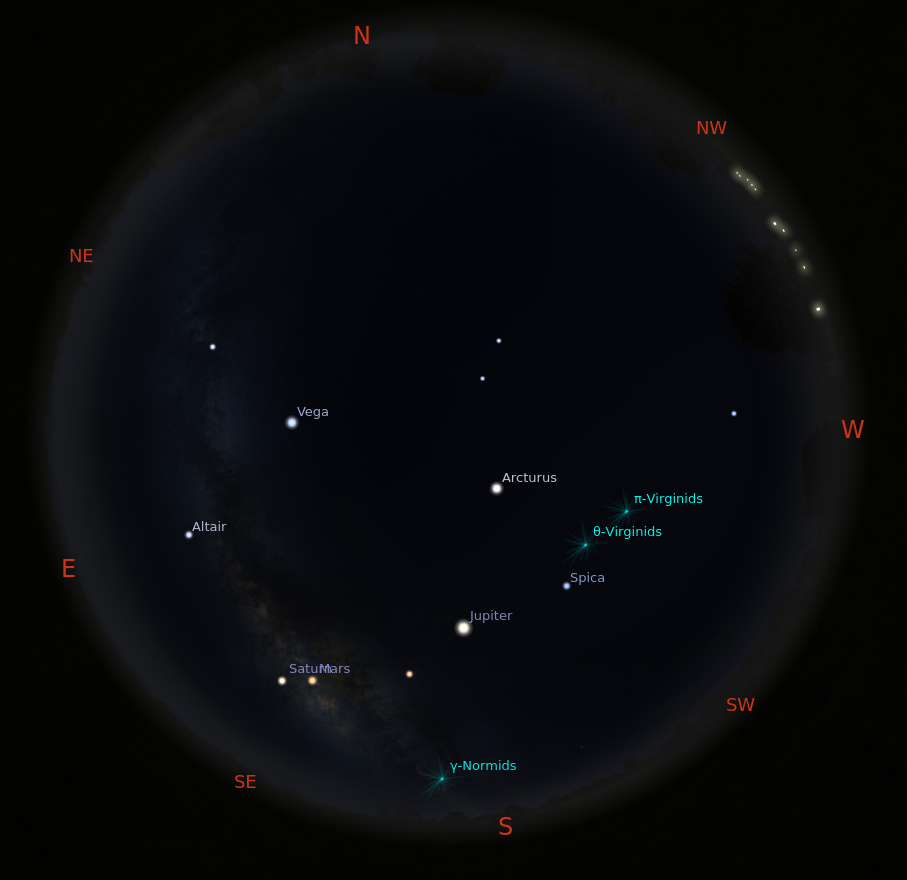
\includegraphics[width=0.6\linewidth]{stellarium.png}
	\caption{Only celestial objects with a magnitude brighter than 2.00 are filtered through for ease of identifying them.}
	\label{fig:stellarium}
\end{figure}

Figure~\ref{stellarium} was then compared to the thresholded video frames of the event in order to try to identify one of the brighter objects. Assuming the stellarium was positioned correctly, celestial objects should appear to be in the same place in both images. Figure~\ref{ThresholdFrame} was the frame that was compared. 

\begin{figure}[ht!]
	\centering
	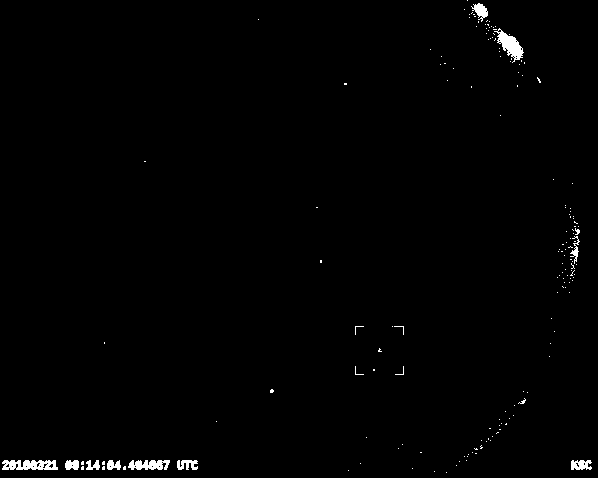
\includegraphics[width=0.5\linewidth]{ThresholdFrame.png}
	\caption{The threshold frame allows one to focus on the easily identifiable, bright, objects in the sky.}
	\label{fig:ThresholdFrame}
\end{figure}

Looking at Figure~\ref{ThresholdFrame} alongside Figure~\ref{stellarium} one can pick out which objects are which. A few pieces of data can be extracted from the two images. The only piece of data that we need is the magnitude of a single object, which can be obtained by clicking on that object in stellarium. For this calibration, Jupiter was used with its magnitude of -2.35 at the time. While only one object is needed, Jupiter and other notable stars are labeled in the identified version of the thresholded frame in Figure~\ref{FrameLabel}.

\begin{figure}[ht!]
	\centering
	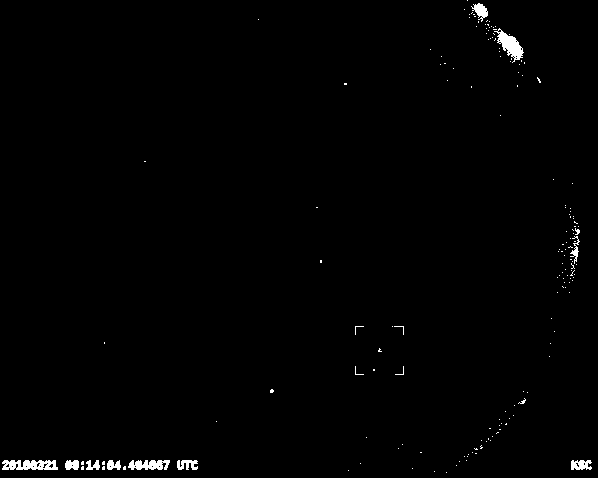
\includegraphics[width=0.5\linewidth]{ThresholdFrame.png}
	\caption{Put Labels on this one, Luke!}
	\label{fig:FrameLabel}
\end{figure}

Another piece of data that can be extracted is that the event in question was most likely from the $\theta$-Virginids or $\pi$-Virginids, as the event is in the same area as those two meteor showers were on that day. This is another piece of strong evidence that the sky is oriented correctly in the images.

Now that we had a celestial object with a magnitude to calibrate to, the program was ran on the event. When it finished, the end result is the magnitude of each frame plotted over the time of the event, showing the light curve of the event. The light curve of this event from the program is shown in Figure~\ref{fig:lightcurve}. 

\begin{figure}[htpb]
	\centering
	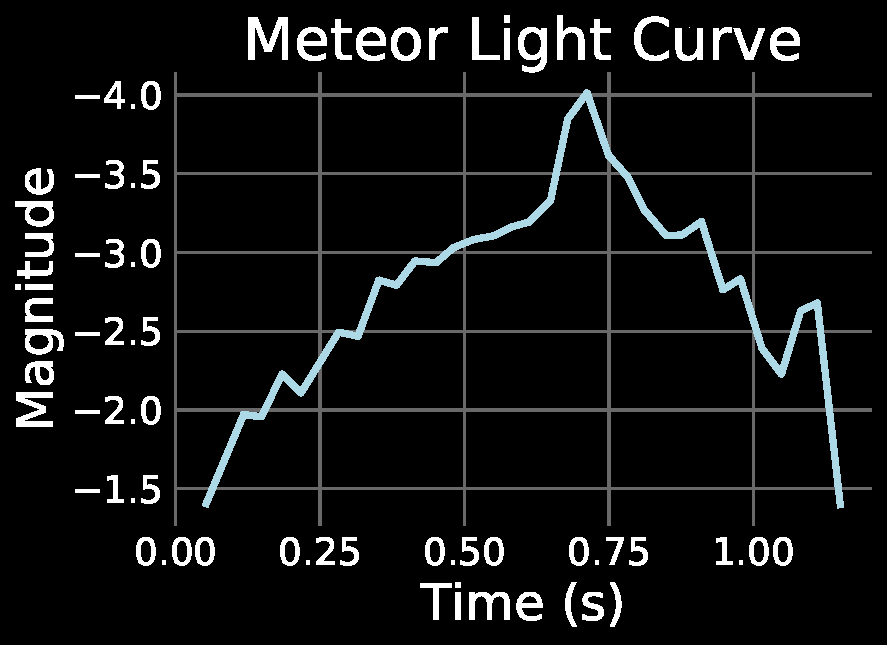
\includegraphics[width=0.6\linewidth]{/home/luke/Data/NASA/2018-03-21-0814/MeteorCurve.pdf}}
	\caption{A lightcurve the program calculated off one of NASA's detected meteor events.}
	\label{fig:lightcurve}
\end{figure}


The general trend shows that program's methodology in calculating the magnitude is sound. We would expect the brightness to gradually grow before diminishing again, and the graph agrees with that. This event in question was detected off from one of NASA's cameras. As a result, we can compare our light curve to NASA's to double check. NASA's light curve can be seen in Figure~\ref{fig:nasa}. They are pretty similar.

\begin{figure}[ht!]
	\centering
	\includegraphics[width=0.6\linewidth]{/home/luke/Data/NASA/2018-03-21-0814/201803210814.pdf}
	\caption{The event in question is the light curve on the top.}
	\label{fig:nasa}
\end{figure}

One aspect of the data that does not seem to fit well is the beginning of the event. This can be seen quantitatively by plotting the residuals of the two data sets and looking for outliers, which is done in Figure~\ref{fig:residuals1}

\begin{figure}[ht!]
	\centering
	\includegraphics[width=0.6\linewidth]{/home/luke/Data/NASA/2018-03-21-0814/201803210814Residuals.pdf}}
	\caption{}
	\label{fig:residuals1}
\end{figure}

The error can also be displayed with the use of a violin plot, shown in Figure~\ref{fig:violinplot}. This allows us to see whether it is overestimating or underestimating the magnitude by looking at the tails of the plot. By focusing the plot's tails, that information is not masked underneath a consistent offset some data may have.

\begin{figure}[ht!]
	\centering
	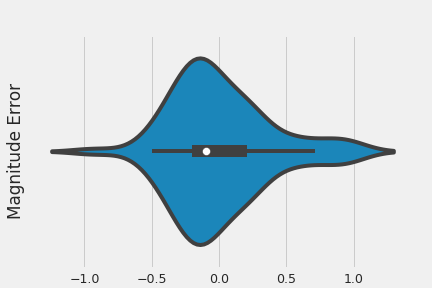
\includegraphics[width=0.6\linewidth]{testviolinplot.png}
	\caption{Testviolinplot}
	\label{fig:violinplot}
\end{figure}

This discrepancy may be because the program does not take into account parameters such as atmospheric extinction. These parameters are more influential if the object moves radially across the night sky in the camera's frame. If NASA did take into account this affect, then that would explain the difference.

\section{Fireballs detected with D6.}

Ultimately, however, the goal of our research is to show our all-sky camera's capabilities. The final test of the photometry script is thus the ability for it to detect new data collected from our own all-sky camera. With self-collected data, however, there are often problems that need to be troubleshooted. One problem that emerged early on in our desire to build an ultra compact and affordable unit was that our hardware was not fast enough to write the frames of the events to the hard drive cleanly. The result of this is incomplete video frames, creating gaps in the data. This can be seen in Figure~\ref{fig:D6Glitch}. 

\begin{figure}[ht!]
	\centering
	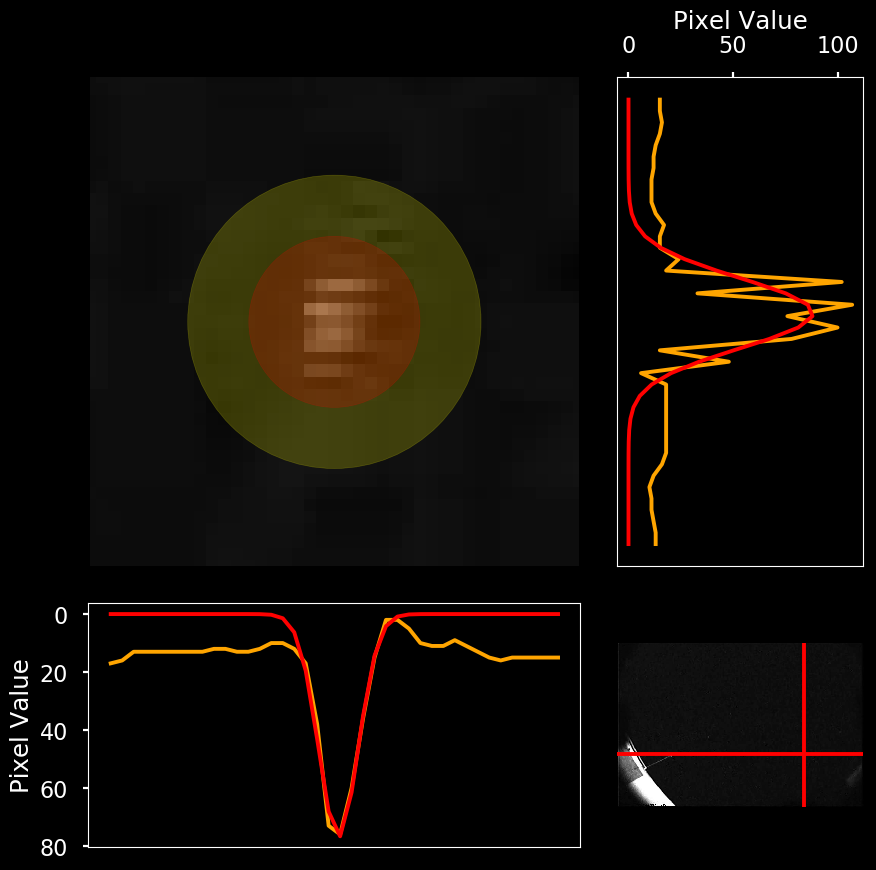
\includegraphics[width=0.6\linewidth]{D6Glitch.png}
	\caption{The incomplete frame data can be seen in both slices of the pixel data.}
	\label{fig:D6Glitch}
\end{figure}

This results in frames with much lower pixel values inside the object's radius than what one would expect, and what it would be if accurately representing the meteoritic phenomenon correctly. This is further seen in the resulting light curve, show in Figure~\refPfig:{D6LightCurve}.

\begin{figure}[ht!]
	\centering
	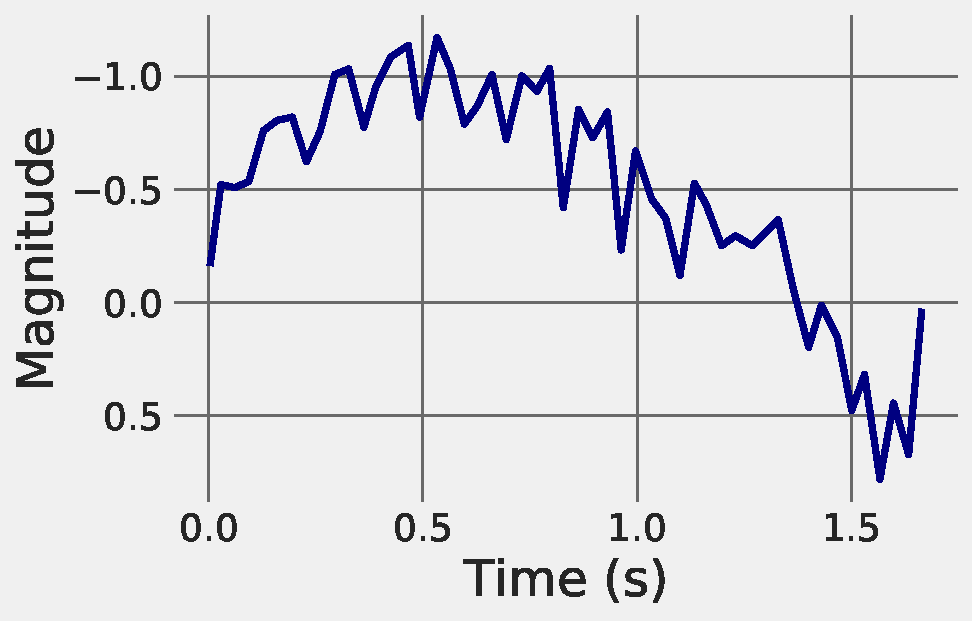
\includegraphics[width=0.6\linewidth]{/home/luke/Data/D6/D6Curve.pdf}
	\caption{The light curve of this event is much less smooth than one would expect from a fireball}
	\label{fig:D6LightCurve}
\end{figure}

%\begin{table}[h!]
  %\centering
  %\begin{tabular}{ | c | m{5cm} | m{5cm} | }
    %\hline
    %my.Lboro & Advantages\\ \hline
    %\begin{minipage}{.5\textwidth}
      %\includegraphics[width=\linewidth, height=60mm]{/home/luke/Data/NASA/2018-03-21-0814/201803210814.pdf}
    %\end{minipage}
    %&
    %%\begin{minipage}[t]{5cm}
      %\begin{itemize}
        %\item Accessibility
        %\item Up to date information
        %\item Fulfil students needs and wants \ldots
      %\end{itemize}
    %%\end{minipage}
    %\\ \hline
  %\end{tabular}
  %\caption{my.Lboro Analysis}\label{tbl:myLboro}
%\end{table}
